\section{Rendu temps-réel}

\begin{frame}[t]{Histoire du rendu temps-réel en 6 images}
  \begin{center}
\includegraphics<1>[height=6cm]{figs/history1.png}
\includegraphics<2>[height=6cm]{figs/history2.png}
\includegraphics<3>[height=6cm]{figs/history3.png}
\includegraphics<4>[height=6cm]{figs/history4.png}
\includegraphics<5>[height=6cm]{figs/history5.png}
\includegraphics<6>[height=6cm]{figs/history6.png}

  \end{center}
\end{frame}

\subsection{Ombrage}

\begin{frame}[t]{Ombrage de Gouraud}
  \begin{itemize}
    \item Dû au mathématicien français Henry Gouraud
    \item Principe : interpolation des intensités lumineuses
    \item Etapes de l'algorithme
    \begin{itemize}
      \item Calcul des normales aux facettes
      \item Calcul des \emph{normales} aux sommets
      \item Calcul des intensités lumineuses aux sommets
      \item Interpolation pour tous les points des facettes
    \end{itemize}
    \item Avantages
    \begin{itemize}
      \item directement implanté sur la GPU
      \item de bons effets visuels sur des surfaces lisses
    \end{itemize}
  \end{itemize}
\end{frame}
%--- Next Frame ---%

\begin{frame}[t]{Principe}
  \begin{center}
    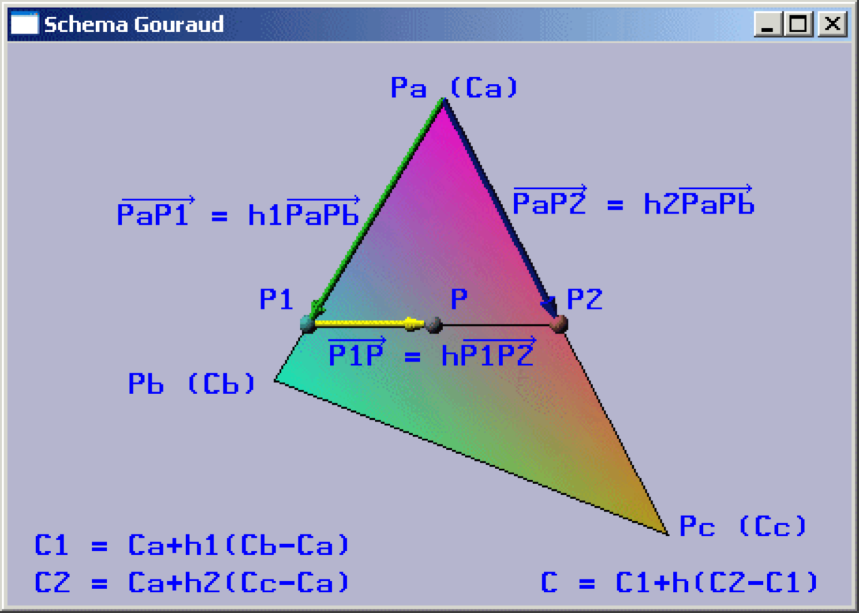
\includegraphics[height=6.5cm]{figs/gouraud1.png}
  \end{center}
\end{frame}

\begin{frame}[t]{Exemple de problème avec le rendu de Gouraud}
  \begin{center}
    \includegraphics<1>[height=4.5cm]{figs/gouraud2.png}
    \includegraphics<2>[height=4.5cm]{figs/gouraud3.png}
    \includegraphics<3>[height=4.5cm]{figs/gouraud4.png}
  \end{center}
  \begin{enumerate}
    \item<1> Calcul des normales
    \item<2> Vue de côté
    \item<3> Vue de dessus
  \end{enumerate}
\end{frame}
%--- Next Frame ---%
%--- Next Frame ---%
%--- Next Frame ---%

\begin{frame}[t]{Ombrage de Phong}
  \begin{itemize}
    \item Algorithme un peu plus avancé que celui de Gouraud
    \item Principe
    \begin{itemize}
      \item Calculer les normales aux facettes
      \item Calculer les \emph{normales} aux sommets
      \item Interpoler les normales en tous les points des facettes
      \item Calculer l'intensité lumineuse en tous points par la loi de Lambert
    \end{itemize}
    \item Avantage
    \begin{itemize}
      \item Permet de rendre certains types de tâches de spécularité
    \end{itemize}
    \item Mais beaucoup plus couteux en temps de calcul
  \end{itemize}
\end{frame}
%--- Next Frame ---%

\begin{frame}[t]{Comparaison entre ombrage de Gouraud et Phong}
  \begin{columns}
\begin{column}{.49\textwidth}
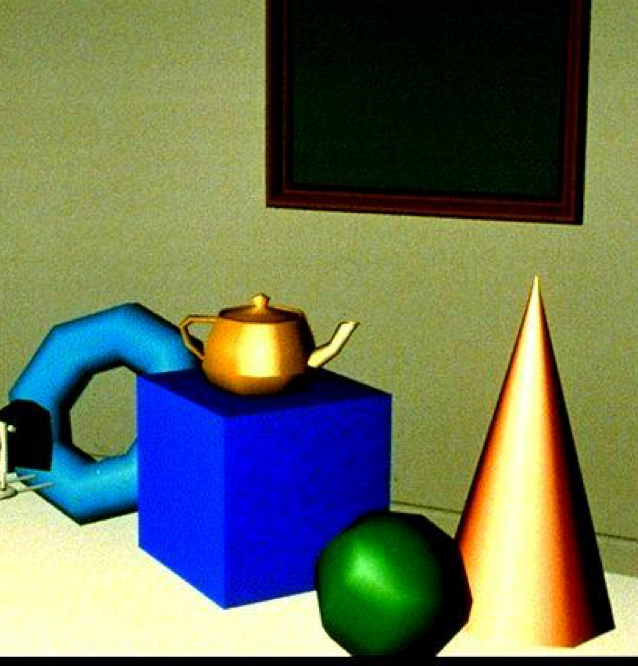
\includegraphics[width=\columnwidth]{figs/exgouraud.png} \\
Gouraud
\end{column}
\begin{column}{.49\textwidth}
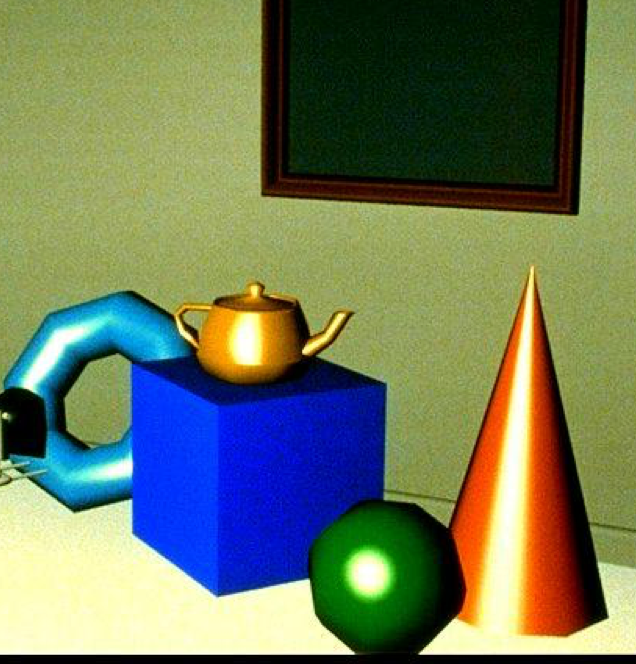
\includegraphics[width=\columnwidth]{figs/exphong.png} \\
Phong
\end{column}
  \end{columns}
\end{frame}
%--- Next Frame ---%

\subsection{Elimination des parties cachées}

\begin{frame}[t]{Elimination des parties cachées : motivation}
  \begin{center}
    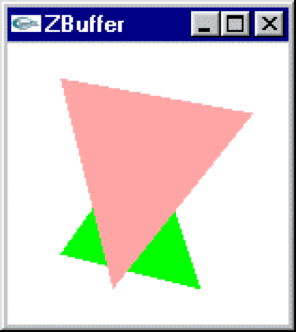
\includegraphics[height=3cm]{figs/peintre1.png}
    \hspace{1cm}
    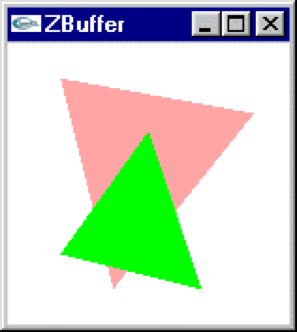
\includegraphics[height=3cm]{figs/peintre2.png}
    \hspace{1cm}
    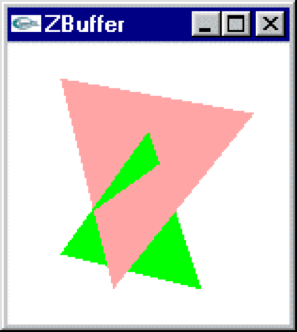
\includegraphics[height=3cm]{figs/peintre3.png}

  \end{center}
\begin{itemize}
  \item Etat de l'art conséquent...
  \item Divers algorithmes dépendant du hardware disponible notamment
\end{itemize}

\end{frame}
%--- Next Frame ---%

\begin{frame}[t]{Algorithme du "peintre"}
  \begin{itemize}
    \item Algorithme de Newell, Newell et Sancha
    \item Principe
    \begin{itemize}
      \item Afficher en commençant par le fond et "peindre" par dessus les objets les plus proches
    \end{itemize}
    \item A partir d'une liste ordonnées de facettes
    \begin{itemize}
      \item  ordonnées par $z_{max}$
      \item afficher par $z_{max}$ décroissant
    \end{itemize}
    \item Problème : comment gérer les facettes qui se coupent ?
  \end{itemize}
\end{frame}
%--- Next Frame ---%

\begin{frame}[t]{Algorithme du z-buffer}
  \begin{itemize}
    \item Idée : stocker l'intensité lumineuse des pixels et leur profondeur
    \item Principe : Si $z$ du pixel < $z$ mémorisée, on mémorise
    \item Avantage : algorithme câblé sur GPU
    \item Inconvénients : taille mémoire requise
  \end{itemize}
\end{frame}

\begin{frame}[t]{Fonctionnement du z-buffer}
  \begin{columns}
    \begin{column}{.49\textwidth}
      \begin{enumerate}
        \item<1-> tous les pixels sont mis à noir et profondeur \emph{infinie}
        \item<2-> Face rouge à $z=4$
        \item<3-> Face jaune à $z=2$
        \item<4-> Face mauve à $z=8$
        \item<5-> Face verte à $z=3$
      \end{enumerate}

    \end{column}
    \begin{column}{.49\textwidth}
      \begin{center}
        \includegraphics<1>[width=\columnwidth]{figs/zbuffer1.png}
        \includegraphics<2>[width=\columnwidth]{figs/zbuffer2.png}
        \includegraphics<3>[width=\columnwidth]{figs/zbuffer3.png}
        \includegraphics<4>[width=\columnwidth]{figs/zbuffer4.png}
        \includegraphics<5>[width=\columnwidth]{figs/zbuffer5.png}
      \end{center}

    \end{column}
  \end{columns}
\end{frame}
%--- Next Frame ---%

\subsection{Textures}

\begin{frame}[t]{Textures}
  \begin{center}
    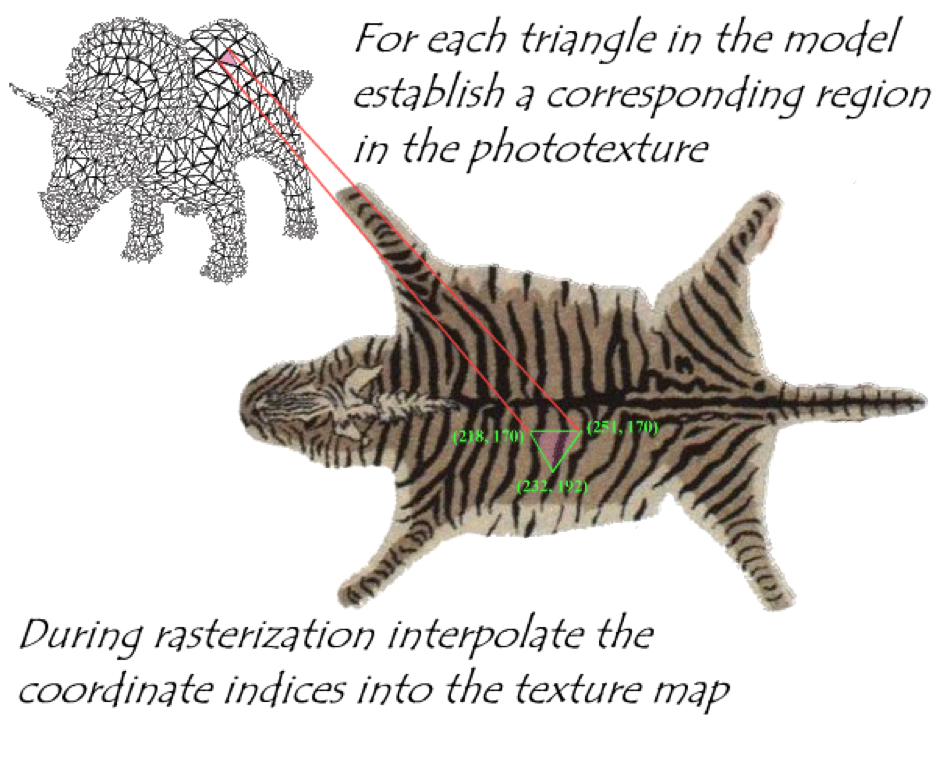
\includegraphics[height=6cm]{figs/textureex.png}
  \end{center}
\end{frame}
%--- Next Frame ---%
%--- Next Frame ---%
\begin{frame}[t]{La quête de "réalisme"}
  \begin{center}
    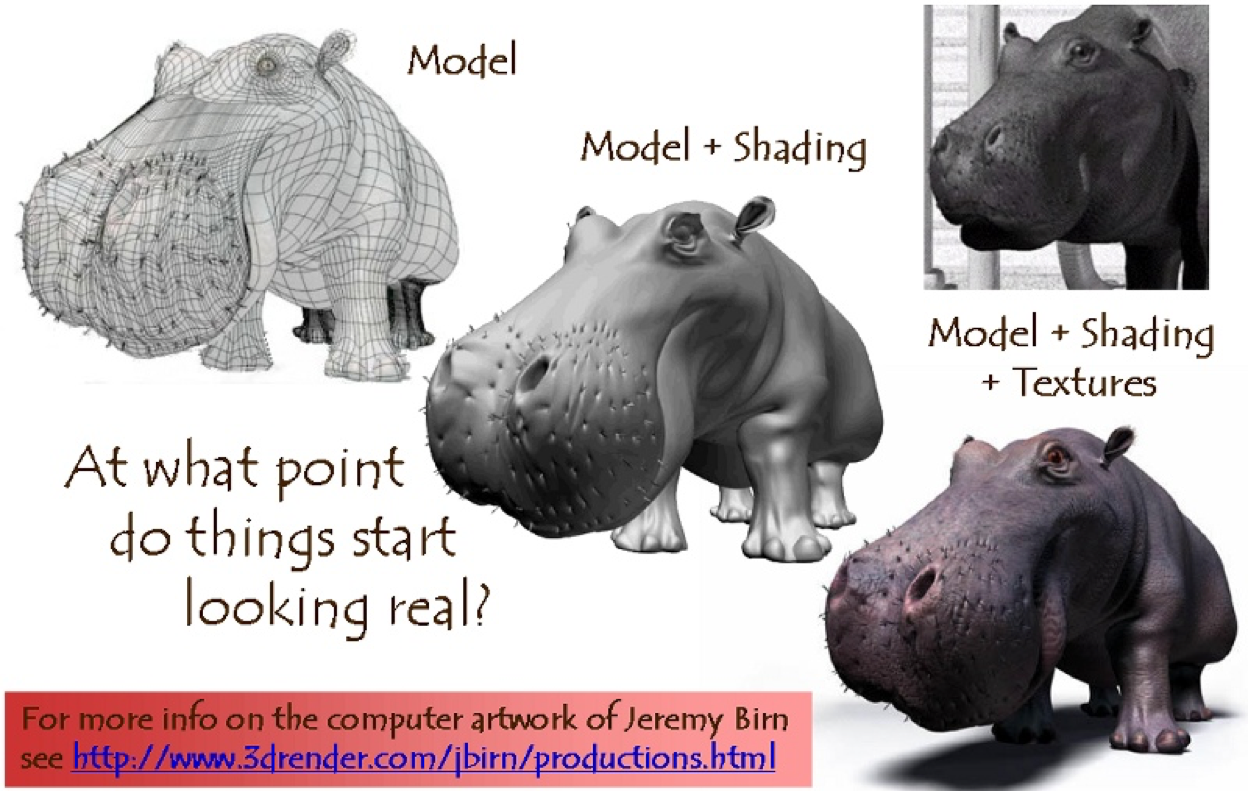
\includegraphics[height=6cm]{figs/textureex2.png}
  \end{center}
\end{frame}

\begin{frame}[t]{Différents types de textures}
  \begin{columns}
\begin{column}{.49\textwidth}
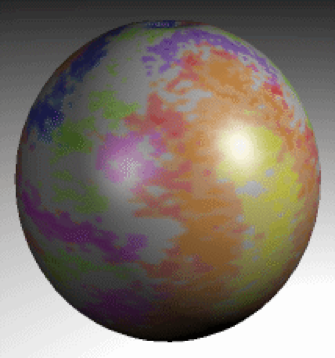
\includegraphics[width=\columnwidth]{figs/cmap.png} \\
Color mapping
\end{column}
\begin{column}{.49\textwidth}
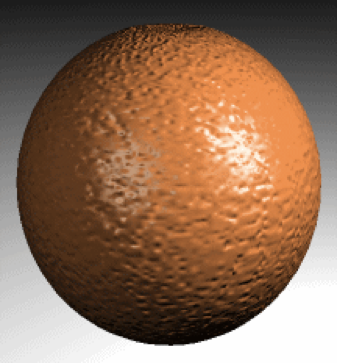
\includegraphics[width=\columnwidth]{figs/bmap.png} \\
Bump mapping
\end{column}
  \end{columns}
\end{frame}

\begin{frame}[t]{Plaquage de textures}
  \begin{itemize}
    \item appelé "texture mapping" en anglais
    \item Image numérique plaquée sur une surface 3D
    \begin{itemize}
      \item Algorithmes directement implantés sur GPU
      \item Sources multiples : scanner, dessin, calcul...
    \end{itemize}
    \item Avantage : meilleur rendu, allègement géométrique
    \item Processus : passer d'un point (3D) de la surface à un point de l'image
    \item Pas si simple
    \begin{itemize}
      \item forme de l'image, problèmes d'aliassage
    \end{itemize}
  \end{itemize}
\end{frame}
%--- Next Frame ---%

\begin{frame}[t]{Différents algorithmes}
\begin{itemize}
  \item En fonction de l'obectif
  \begin{center}
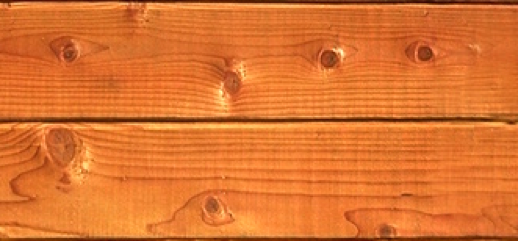
\includegraphics[height=2cm]{figs/parquet.png}
\hspace{1cm}
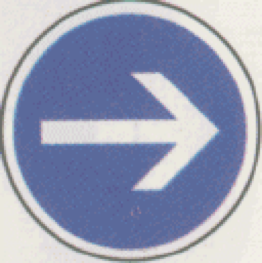
\includegraphics[height=2cm]{figs/panneau.png}
\hspace{1cm}
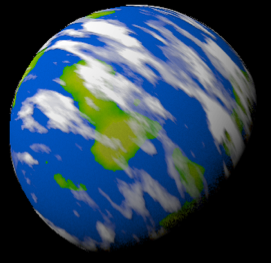
\includegraphics[height=2cm]{figs/planete.png}
  \end{center}
  \item \emph{mipmapping} : utiliser plusieurs textures de résolution différentes
  \begin{center}
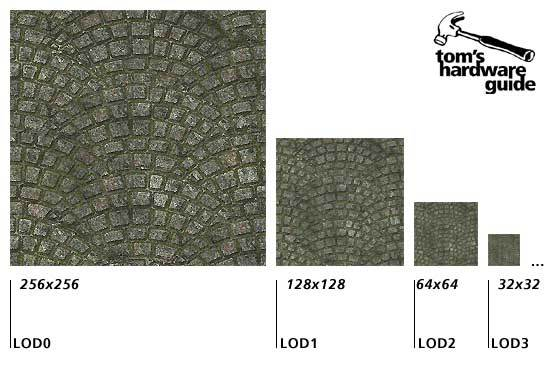
\includegraphics[height=3.5cm]{figs/mipmaps.jpg}
  \end{center}
\end{itemize}
\end{frame}

\begin{frame}[t]{Billboards}
  \begin{columns}
\begin{column}{.49\textwidth}
  \begin{itemize}
    \item Objets texturés "auto-orientables" sur l'axe vertical
    \item Avantage
    \begin{itemize}
      \item Moyen simple de ne reproduire qu'une face d'un objet éloigné
    \end{itemize}
    \item Inconvénients
    \begin{itemize}
      \item Pas adapté au survol
      \item temps de calcul
    \end{itemize}
  \end{itemize}
\end{column}
\begin{column}{.49\textwidth}
\begin{center}
  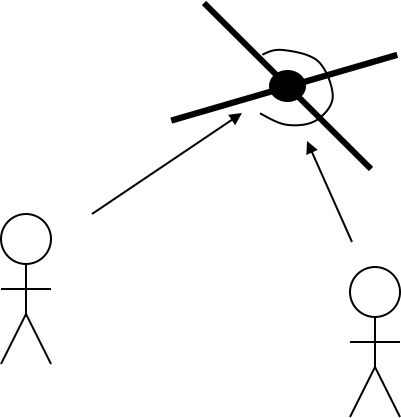
\includegraphics[height=3.5cm]{figs/billboard.png}
\end{center}
\end{column}
  \end{columns}
\end{frame}
%--- Next Frame ---%
\subsection{Aliasing}

\begin{frame}[t]{Aliassage (aliasing)}
  \begin{center}
    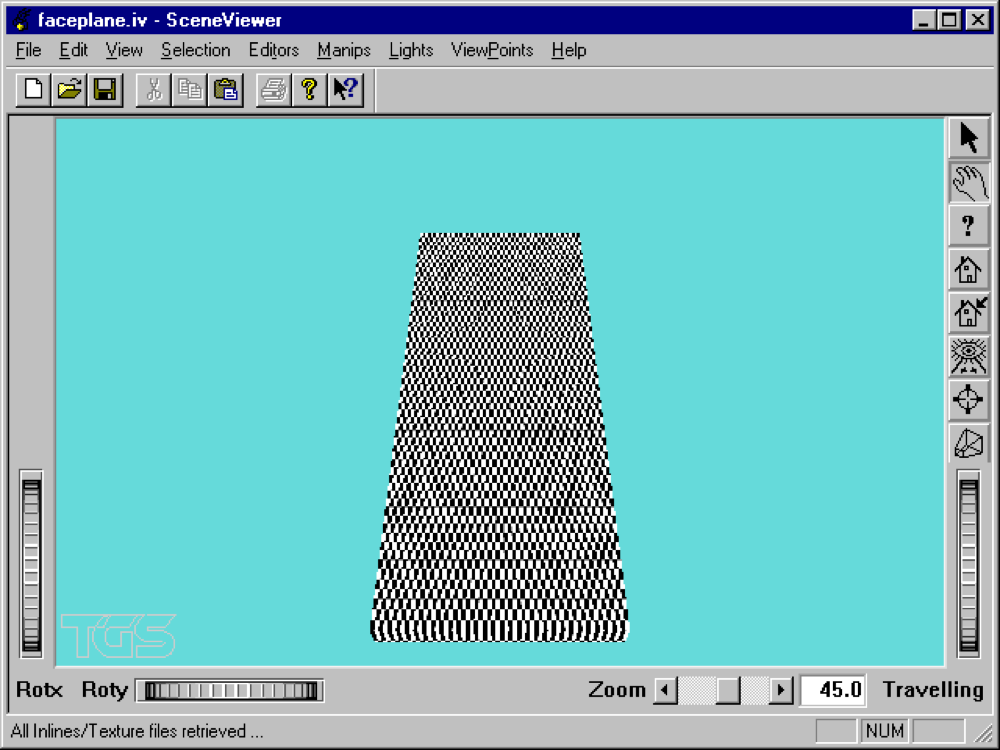
\includegraphics[height=6cm]{figs/alias1.png}
  \end{center}
\end{frame}
%--- Next Frame ---%

\begin{frame}[t]{Effets de l'aliassage}
  \begin{columns}
    \begin{column}{.49\textwidth}
      \begin{itemize}
        \item Effets d'escaliers
        \item Petits objets entièrement ou partiellement masqués
        \item Effets de moirés
        \item Causes : théorie du signal
        \begin{itemize}
          \item Recouvrement du spectre
          \item Dû à l'échantillonnage
        \end{itemize}
      \end{itemize}
    \end{column}
    \begin{column}{.49\textwidth}
      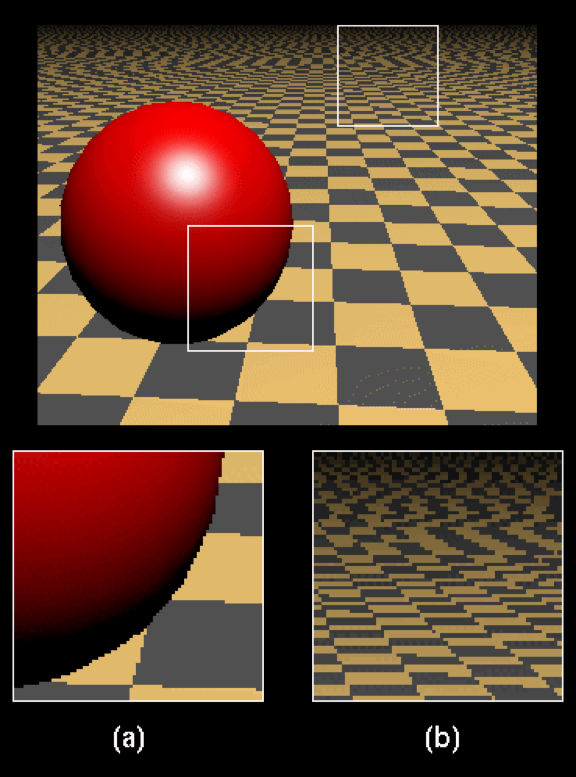
\includegraphics[width=.9\columnwidth]{figs/alias2.png}
    \end{column}
  \end{columns}
\end{frame}
%--- Next Frame ---%

\begin{frame}[t]{Anti-aliasing}
  \begin{itemize}
    \item Constat : problème de représentation des hautes fréquences
    \item Solution 1 : augmenter la fréquence d'échantillonnage
    \begin{itemize}
      \item Très couteux (2D)
    \end{itemize}
    \item Supprimer les hautes fréquences dans les images
    \begin{itemize}
      \item par augmentation locale de l'échantillonnage puis lissage
      \item grosso modo ce que font les GPU
    \end{itemize}
    \item Echantillonnage stochastique : bruit moins perceptible que les défauts réguliers
  \end{itemize}
\end{frame}
  %--- Next Frame ---%


\begin{frame}[t]{Exemple}
  \begin{center}
    \includegraphics<1>[height=3.5cm]{figs/alias3.png}
    \includegraphics<2>[height=7cm]{figs/alias4.png}
    \includegraphics<3>[height=3.5cm]{figs/alias3.png}
    \hspace{0.5cm}
    \includegraphics<3>[height=3.5cm]{figs/alias5.png}

  \end{center}
\end{frame}
%--- Next Frame ---%

\begin{frame}[t]{Exemple 2 : lissage des polices}
  \begin{center}
    
\includegraphics[height=6cm]{figs/truetype.png}
  \end{center}
\end{frame}

\subsection{Niveaux de détail}

\begin{frame}[t]{Niveaux de détail (LoD)}
  \begin{itemize}
    \item Un noeud spécial dans le graphe de scène qui possède plusieurs fils
    \item Un seul est affiché à la fois en fonction d'un critère
    \begin{itemize}
      \item généralement la distance de l'objet à l'observateur
    \end{itemize}
  \end{itemize}
  \begin{center}
    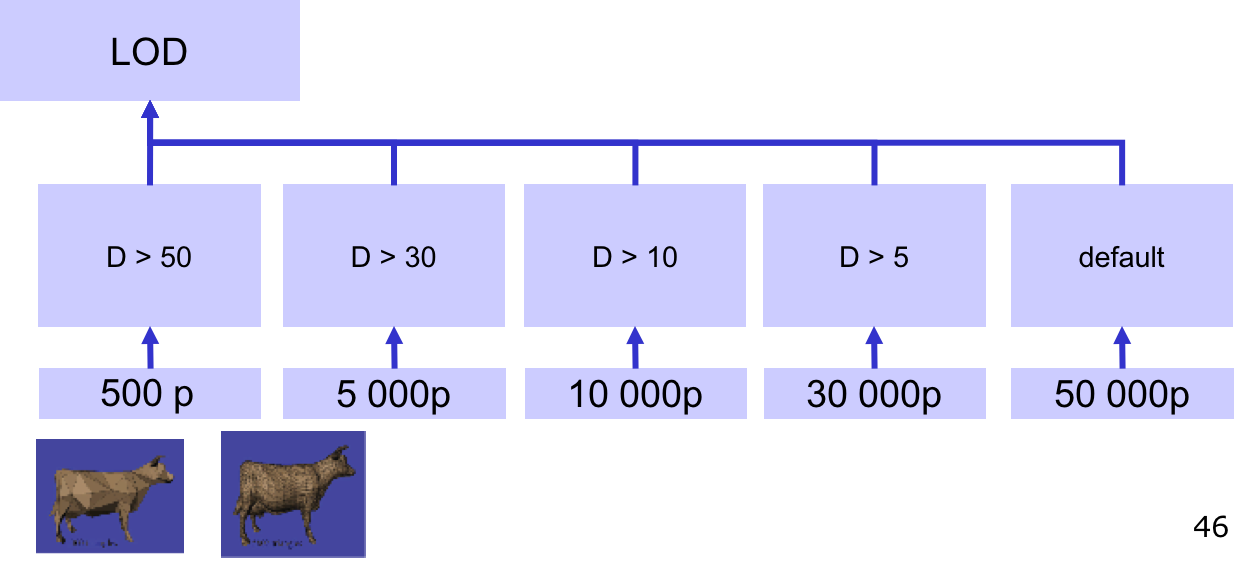
\includegraphics[height=4.5cm]{figs/lodth.png}
  \end{center}
\end{frame}
%--- Next Frame ---%
